\documentclass[sigconf]{acmart}
\settopmatter{printacmref=false, printccs=false, printfolios=true}
\renewcommand\footnotetextcopyrightpermission[1]{}
% the header otherwise shows acmart's placeholder venue (Conference'17, Washington)
\acmConference[ComPar 2026/27]{Computação Paralela, Project 1}{November 2026}{NOVA FCT, Portugal}

\usepackage{booktabs} % For formal tables
\usepackage{graphicx}
\graphicspath{ {./images/} }

\usepackage[acronym, automake]{glossaries-extra}
\setabbreviationstyle[acronym]{long-short}
\makeglossaries
\newacronym{aqe}{AQE}{Adaptive Query Execution}
\newacronym{smj}{SMJ}{Sort-Merge Join}
\newacronym{bhj}{BHJ}{Broadcast Hash Join}
\newacronym{jvm}{JVM}{Java Virtual Machine}
\newacronym{tlc}{TLC}{NYC Taxi and Limousine Commission}
\newacronym{os}{OS}{Operating System}


\renewcommand{\topfraction}{0.9}
\renewcommand{\dbltopfraction}{0.9}
\renewcommand{\textfraction}{0.07}
\setcounter{topnumber}{3}
\setcounter{dbltopnumber}{2}

\begin{document}
\title{Performance Engineering of a PySpark Pipeline on NYC Taxi Trips}

\author{Gabriel Matias Falcão (77390)}
\affiliation{%
      \institution{NOVA School of Science and Technology, Universidade NOVA de Lisboa}
      \city{Lisbon}
      \country{Portugal}}

\begin{abstract}
      This report presents the profiling and optimisation of a PySpark pipeline that
      processes 29.7\,M NYC yellow-taxi trips (three mandatory operations plus
      origin-destination flows and trip-type classification). Each report's structure
      follows a profile, hypothesise, optimise, measure loop, sort-merge joins
      against tiny tables, spills in under-partitioned reduce stages and repeated
      scans are identified as the main weights of the baseline. Optimisations include
      broadcast joins, writing results once, materialising the cleansed data and
      explicitly partitioning a cached result, which cut individual operations by up
      to 5$\times$; caching the wrong DataFrames and smaller scan splits are reported
      as measured failures. Execution time scales sub-linearly with input size
      because of a fixed cost ($\sim$39\,s on the Docker cluster, $\sim$25\,s
      locally), and a single-machine Docker cluster shows why adding executors on
      shared hardware does not help.
\end{abstract}

\keywords{Apache Spark, performance engineering, query plans, broadcast join, caching}

\maketitle

\section{Introduction}

The pipeline processes the \gls{tlc} yellow taxi trip records~\cite{tlc}: one
parquet file per month plus a 265-row zone lookup table. Development and all
measurements use 2026-01..08 (29.7\,M records, 488\,MB of parquet). Besides the
mandatory operations (M1 cleaning statistics, M2 temporal aggregation per
borough, day and hour, M3 monthly zone statistics with rolling windows), two
optional ones were chosen for the bottlenecks they expose. \textbf{O2}
(origin-destination flows) joins the zone table twice and derives three outputs
(route shares, top-20 per borough, Q1/Q3 reversals) from one monthly aggregate,
so it stresses multi-way joins and recomputation. \textbf{O4} (trip-type
classification) aggregates trips into at most 263\,$\times$\,24 buckets and
joins that small result back to every trip, the shape where join strategy and
hot-zone skew decide the cost.

Every operation joins $\sim$21\,M trips with a tiny table and aggregates, so
the cost is how Spark moves and re-reads data, not arithmetic. Code, logs and
per-optimisation reports are in the repository~\cite{repo}.

\section{Pipeline}

All operations share two steps. \emph{Load} groups the files by physical
parquet schema (2026 has two variants), casts each group to the documented
schema with \texttt{try\_cast} and combines them with \texttt{unionByName}.
\emph{Clean} keeps a record only if it passes the M1 rules: no null in a used
column, fare and distance $>0$, 1--6 passengers, dropoff after pickup, location
ids in 1--263 (20.95\,M records remain). Each operation then joins the zone
table and aggregates; M3 and O2 add windows, O2 a pivot, O4 a second
aggregation after the join back.

Design decisions: the DataFrame API is used throughout, because operations are
composed in Python from shared pieces (cleaning rules, zone joins, feature
flags), and it compiles to the same Catalyst plans as SQL; no UDFs are used, so
no work goes through Python workers; timestamps are read as
\texttt{timestamp\_ntz} with the session zone fixed to UTC, so hours and
weekdays do not depend on the host; routes and zones are keyed by id because
zone names are not unique. In the baseline \texttt{spark.sql.\allowbreak
      autoBroadcast\allowbreak JoinThreshold=-1}, so every join starts as a \gls{smj}
and each optimisation is an explicit, measured feature flag.
Figure~\ref{fig:plan} shows the physical plan of M2.

\begin{figure*}[t]
      \centering
      \Description{Two simplified physical plans of M2 side by side: the baseline with a sort-merge join and an exchange of all trips, and the optimised plan with a broadcast hash join and no trip exchange.}
      \begin{minipage}[t]{0.5\textwidth}
            \scriptsize \begin{verbatim}
HashAggregate (final)
+- Exchange (Borough, day, hour)
   +- HashAggregate (partial)
      +- SortMergeJoin PULocationID=LocationID
         :- Sort
         :  +- Exchange (PULocationID) <- all trips
         :     +- Union (2 schema groups)
         :        :- Project(try_cast) / Filter
         :        :  +- Scan parquet [7 cols]
         :        +- Project(try_cast) / Filter
         :           +- Scan parquet [7 cols]
         +- Sort
            +- Exchange (LocationID)
               +- Scan csv (zones)
\end{verbatim}
      \end{minipage}%
      \begin{minipage}[t]{0.47\textwidth}
            \scriptsize \begin{verbatim}
HashAggregate (final)
+- Exchange (Borough, day, hour)
   +- HashAggregate (partial)
      +- BroadcastHashJoin BuildRight
         :- Union (2 schema groups)
         :  :- Project(try_cast) / Filter
         :  :  +- Scan parquet [7 cols]
         :  +- Project(try_cast) / Filter
         :     +- Scan parquet [7 cols]
         +- BroadcastExchange
            +- Scan csv (zones)
\end{verbatim}
      \end{minipage}
      \caption{M2 physical plan (\texttt{explain("formatted")}, simplified). Left:
            baseline, every cleaned trip is shuffled and sorted to join 265 rows. Right:
            after broadcasting the zone table (Section~\ref{sec:bhj}).}
      \label{fig:plan}
\end{figure*}

\section{Profiling and Baseline}
\label{sec:baseline}

\textbf{Setup.} Laptop with an Intel i7-1195G7 (4 cores / 8 threads), 15\,GiB
RAM; Spark 4.2.0 (PySpark), OpenJDK 25, Python 3.14, \texttt{local[*]} (8 cores),
\texttt{spark.driver.memory=2g}; non-default configuration: no automatic
broadcast, session time zone UTC. \gls{aqe}~\cite{spark-tuning} is on with the
default 200 shuffle partitions.

\textbf{Method.} Each configuration runs 3 times; reported times are medians.
Outputs go to Spark's \texttt{noop} sink, because \texttt{show()} computes only
the rows it prints. Every run logs \texttt{explain("formatted")} and \texttt{explain(True)},
and the Lab 3 profiler records jobs, stages, tasks, shuffle and spill per
operation. Per-stage task-time quantiles come from the Spark UI REST API\cite{spark-api}.
Spark's input metric reports 6\,MiB for scans that read 383\,MiB of parquet column
chunks, so input volume is taken from the parquet footers instead.

\begin{table}[!t]
      \centering
      \footnotesize
      \setlength{\tabcolsep}{3pt}
      \begin{tabular}{lrrrrr}
            \toprule Op & Wall (s) & Stages & Tasks & Shuffle read & Spill mem / disk    \\
            \midrule M1 & 14.5     & 8      & 76    & 5.4\,KB      & 0                   \\
            M2          & 45.7     & 18     & 152   & 953.8\,MB    & 1.9\,GB / 832.6\,MB \\
            M3          & 21.1     & 9      & 76    & 318.5\,MB    & 768\,MB / 261\,MB   \\
            O2          & 20.3     & 81     & 515   & 53.9\,MB     & 0                   \\
            O4          & 22.1     & 18     & 220   & 222.4\,MB    & 704\,MB / 107\,MB   \\
            \bottomrule
      \end{tabular}
      \caption{Baseline, median of 3 runs (stage, task and shuffle counts identical
            in all runs).}
      \label{tab:baseline}
\end{table}

\textbf{Bottlenecks.} (1)~\emph{Trip-side shuffle of the \gls{smj}}: every
operation hashes and sorts all $\sim$21\,M cleaned trips to join a table of $\le$\,6\,312
rows (Figure~\ref{fig:plan}, left). The stage after that shuffle is the most expensive
of each operation and holds all of the spill (M2 stage 14: 476\,MB read, 896\,MB
/ 392\,MB spilled, 99\,s of task time). (2)~\emph{Too few reduce partitions}: \gls{aqe}
coalesces the 200 shuffle partitions into 9, so each task sorts $\sim$53\,MB
and spills, and 9 tasks run on 8 cores in two waves, the 9th alone for $\sim$12\,s.
(3)~\emph{Recomputation}: M2's display and parquet write are two actions, so its
scan and join run twice (stages 11/14 rerun as 20/23, half of its shuffle); O2
rescans the trips for each of its 3 outputs and O4 scans them twice. (4)~\emph{Skew}:
not found, the slowest reduce task is at most 1.1$\times$ the median, because \gls{aqe}
packs many zones into each partition. (5)~\emph{Column pruning}: already
done by Catalyst, which pushes the projection into the scan (7 of 20 columns
read); selecting the used columns explicitly (\texttt{-{}-prune-column})
leaves the \texttt{ReadSchema} unchanged. Three of the seven columns are read
only for the cleaning rules, which Section~4.3 removes.

\section{Optimisation Study}

\begin{table*}[!t]
      \centering
      \footnotesize
      \begin{tabular}{p{3.0cm}p{4.4cm}p{9.2cm}}
            \toprule Optimisation              & Bottleneck addressed                        & Measured impact (median wall time)                                                                                                                                                   \\
            \midrule Broadcast joins           & Trip shuffle + sort of the \gls{smj}, spill & M2 45.7$\to$20.9\,s, M3 21.1$\to$11.8\,s, O4 22.1$\to$15.6\,s; spill 1.9\,GB$\to$0                                                                                                   \\
            Cache shared results               & Trips scanned once per action               & O2 21.7$\to$17.0\,s; M2 and O4 slower, kept for O2 only                                                                                                                              \\
            Smaller scan splits                & Uneven scan tasks                           & No gain, parallelism capped by 32 row groups                                                                                                                                         \\
            Write once (M2)                    & Result computed twice                       & M2 23.0$\to$15.3\,s, one scan stage less                                                                                                                                             \\
            Clean once, read many              & Re-scan, cast and clean per operation       & M2 13.8$\to$9.0\,s, M3 13.4$\to$6.8\,s, O2 19.0$\to$16.3\,s, O4 13.9$\to$7.9\,s; all ops 96.2$\to$92.3\,s incl.\ write                                                               \\
            Coalesce O2 cache                  & 200 tiny tasks per cache read               & O2 24.2$\to$14.8\,s (run alone), tasks 2\,443$\to$370                                                                                                                                \\
            \midrule All applied (one session) &                                             & M2 38.3$\to$7.7\,s (5.0$\times$), M3 18.2$\to$7.4\,s (2.5$\times$), O2 18.4$\to$9.8\,s (1.9$\times$), O4 21.0$\to$8.6\,s (2.4$\times$); all ops 136.8$\to$76.9\,s incl.\ clean write \\
            \bottomrule
      \end{tabular}
      \caption{Summary of the optimisations; each row is measured against the configuration
            with the rows above it applied, in its own report. The last row comes from
            one session that ran every cumulative configuration 3 times (Figure~\ref{fig:cumulative}).}
      \label{tab:summary}
\end{table*}

Optimisations are cumulative: each one is measured against the configuration
that includes the previous ones, with all other settings unchanged.
Table~\ref{tab:summary} summarises them, and Figure~\ref{fig:cumulative}
re-measures the whole path in a single session (3 runs per configuration, each
started on an idle machine), so the steps are directly comparable. It also
shows that caching O2 alone did not pay off inside a full run (16.9\,s $\to$
18.6\,s); only the coalesced cache did (9.8\,s).

\begin{figure}[!t]
      \centering
      \Description{Grouped bar chart of wall time for M2, M3, O2 and O4 across five cumulative configurations, falling from 18 to 38 seconds at baseline to 7 to 10 seconds at the end.}
      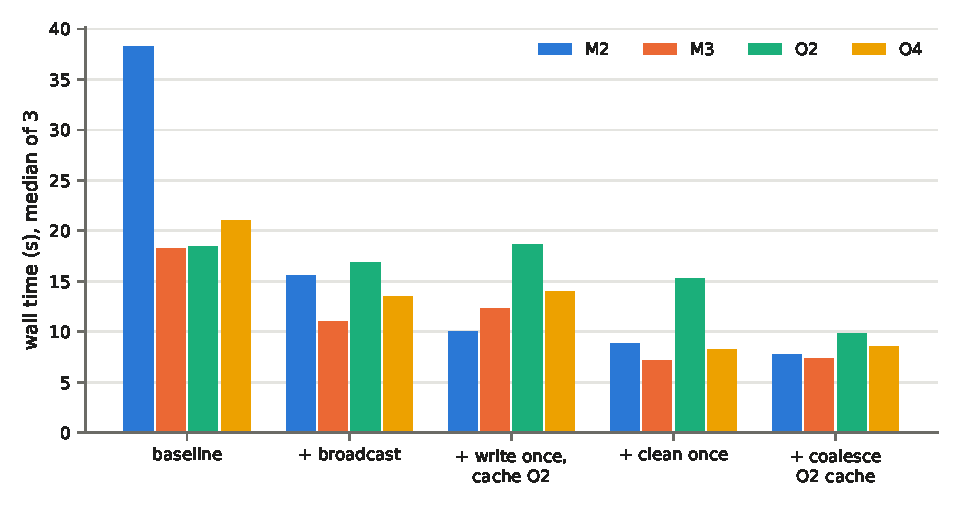
\includegraphics[width=\columnwidth]{cumulative.pdf}
      \caption{Wall time per operation across the cumulative optimisations, one
            session, median of 3 runs of all operations.}
      \label{fig:cumulative}
\end{figure}

\subsection{Broadcast the small side of every join}
\label{sec:bhj} \emph{Bottleneck:} the trip-side \texttt{Exchange} and sort of
the \gls{smj} and the spill after it (Section~\ref{sec:baseline}). \emph{Hypothesis:}
the zone table (265 rows) and O4's bucket table ($\le$\,6\,312 rows) fit in every
executor, so a \gls{bhj} can probe them inside the scan tasks and the trips never
need to be shuffled. \emph{Change:} \texttt{-{}-broadcast-join} wraps the
small side in a \texttt{broadcast()} hint~\cite{spark-tuning}. \emph{Result:} every
\texttt{SortMergeJoin} becomes a \texttt{BroadcastHashJoin} (Figure~\ref{fig:plan},
right), the 9-task reduce stage disappears, and only partial aggregates are
shuffled. Shuffle read falls from 953.8\,MB to 1.5\,MB for M2 (318.5\,MB to
0.7\,MB for M3, 222.4\,MB to 1.8\,MB for O4), all spill goes to zero, and M2, M3
and O4 run 2.2$\times$, 1.8$\times$ and 1.4$\times$ faster. O2 does not change,
because its joins run on aggregated routes rather than trips.

\subsection{Reusing results: cache versus write once}
\emph{Bottleneck:} with the shuffles gone, the scans dominate, and multi-action
operations scan the trips once per action (M2 twice, O2 three times, O4 twice).
\emph{Hypothesis:} persisting the shared DataFrame leaves one scan per
operation. \emph{Change:} \texttt{-{}-cache-dataframe} caches M2's result, O2's
monthly routes and O4's cleaned trips. \emph{Result:} only O2 improves (21.7\,s
$\to$ 17.0\,s, 1.28$\times$): its cache is a 4.8\,MiB aggregate, so two of
three scans disappear cheaply. M2 gets slower (20.9\,s $\to$ 23.2\,s): the
cached result keeps all 200 shuffle partitions, which \gls{aqe} would
otherwise coalesce into one, so the write runs 200 tasks and produces 663 files
instead of 6. O4 also gets slower (15.6\,s $\to$ 19.9\,s): building a 390\,MiB
in-memory cache of 21\,M trips adds 41\,s of task time to the scan, more than the
second parquet scan it replaces. The cache was therefore kept for O2 only. For
M2 the fix is to \textbf{write once} (\texttt{-{}-write-once}): write the
parquet output first and display the 967-row result read back from it. One of the
two 18-task scan stages disappears, task time drops by 37\,\% and M2 goes from
23.0\,s to 15.3\,s (1.5$\times$), with identical output.

\subsection{Clean once, read many}
\emph{Bottleneck:} every operation still starts with a \texttt{Union} of two
scans, each with \texttt{try\_cast} projections and a 13-predicate cleaning
filter; a run of all operations does this 9 times on the same rows and also reads
columns used only by the cleaning rules. \emph{Hypothesis:} materialising the cleaned,
typed trips once as parquet removes that work from every operation, at the cost
of one write; in-memory caching was ruled out by the O4 result and by the 2016--2020
data size. \emph{Change:} \texttt{-{}-materialise-clean} writes the cleaned
trips (9 columns, 8\,MiB row groups, 324\,MiB) and runs M2--O4 on that copy;
M1 still reads the raw files. \emph{Result:} \texttt{Union} nodes drop from 9 to
1 and parquet scans from 18 to 10; M2's scan reads 5 columns with one pushed
filter instead of 7 with 13. Task time falls by 41\,\% (M2), 60\,\% (M3), 19\,\%
(O2) and 48\,\% (O4). The one-time write costs 19.4\,s, yet a run of all
operations already drops from 96.2\,s to 92.3\,s including it, and to 72.5\,s once
the copy exists. A \texttt{DISK\_ONLY} persist of the same data was also
measured: it builds 4.4\,s slower (21.4\,s versus 17.0\,s), reads are within
noise, and unlike the parquet copy it is lost when the application ends.

\subsection{Partition the O2 cache explicitly}
\label{sec:coalesce} \emph{Bottleneck:} O2 is now the slowest operation, and its
time is mostly fixed: 10.6\,s on one month of data, 15.8\,s on eight (Section~\ref{sec:analysis}).
Its three outputs read the 4.8\,MiB route cache in five 200-task stages whose
tasks take 12--132\,ms (median); these stages hold 74\,s of O2's 128\,s of
task time. \emph{Hypothesis:} the cache freezes the 200 shuffle partitions of
the window that produces the routes, and \gls{aqe} coalesces partitions when
reading a shuffle but not when reading a cache, so each output pays task overhead
for $\sim$25\,KB partitions (the same mechanism that slowed M2's cache in Section~4.2).
\emph{Change:} \texttt{-{}-coalesce-cache} coalesces the routes to the default
parallelism (8) before caching, without a shuffle. \emph{Result:} tasks drop
from 2\,443 to 370, the five stages run 8 tasks of 0.3--1.7\,s with 39\,s
instead of 74\,s of task time, and O2 goes from 24.2\,s to 14.8\,s (1.64$\times$,
O2 run alone) with identical output. Smaller scan splits (\texttt{max\allowbreak
      Partition\allowbreak Bytes}) gave no gain: the raw files hold only 32 row
groups, which splits cannot divide~\cite{parquet-format,spark-parquet}.

\section{Analysis}
\label{sec:analysis}

No multi-node cluster was available, so all cluster results come from a
Docker standalone cluster~\cite{spark-standalone} on the same laptop (one
master, workers of 2 cores / 2\,GiB, driver in its own container), measured in
a single session with the final configuration; \texttt{local[*]} runs
supplement them.

\textbf{Dataset scale.} On 3 workers, the pipeline was run on 10, 20 and 50\,\%
samples (the method suggested by the assignment) and on 1, 2, 4 and 8 month
files (Figure~\ref{fig:scale}). Time grows sub-linearly: 8$\times$ more input
costs only 2.3$\times$ more time (47.2\,s $\to$ 110.7\,s). A straight line
through the month series, $T \approx 39\,\mathrm{s}+ 73\,\mathrm{s}\cdot f$,
shows that about 39\,s of every run is fixed: scheduling the $\sim$10 actions
per run on the executors, their warm-up, and O2's small cached stages. Locally
the same fit gives $25\,\mathrm{s}+66\,\mathrm{s}\cdot f$, so the cluster adds
mostly fixed cost. The data-dependent part is linear, because after the
optimisations no trip rows are shuffled. Sampling understates small inputs:
\texttt{sample()} drops rows after the scan, so a 10\,\% sample (55.9\,s) is
slower than a real 12.5\,\% input (47.2\,s).

\begin{figure}[!t]
      \centering
      \Description{Line chart of wall time against dataset fraction for month files and samples, both above a dashed linear-scaling line at small fractions.}
      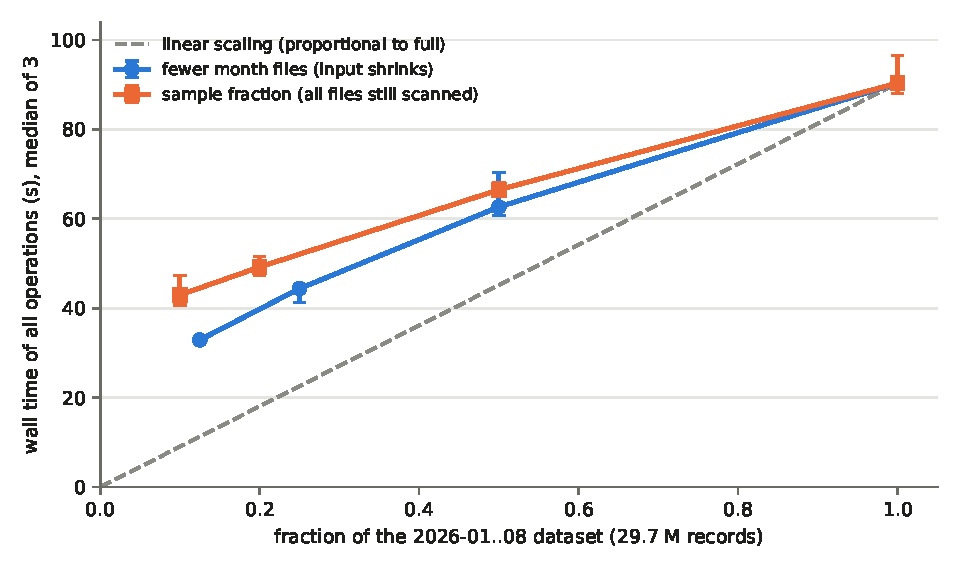
\includegraphics[width=\columnwidth]{scale.pdf}
      \caption{Wall time of all operations versus dataset fraction (median of 3,
            bars: min--max), final configuration, 3-worker Docker cluster.}
      \label{fig:scale}
\end{figure}

\textbf{Cluster size.} With the full data (Table~\ref{tab:docker}), every added
worker makes the run slower. The extra cores are not extra hardware: the same
work costs more task time as executors are added (M3 13\,s with one worker,
39\,s with three), because

\begin{table}[!t]
      \centering
      \footnotesize
      \begin{tabular}{rrrrr}
            \toprule
            Workers & Cores & Wall (s), median [min--max] & Speedup & Efficiency \\
            \midrule
            1       & 2     & 85.7 [84.2--86.7]           & 1.00    & 1.00       \\
            2       & 4     & 92.5 [91.0--93.7]           & 0.93    & 0.46       \\
            3       & 6     & 110.2 [108.8--110.8]        & 0.78    & 0.26       \\
            \bottomrule
      \end{tabular}
      \caption{Docker standalone cluster on one laptop (4 cores / 8 threads),
            all operations, 3 runs per size. Speedup and efficiency relative to
            1 worker. For reference, \texttt{local[*]} takes 76.9\,s.}
      \label{tab:docker}
\end{table} 6 executor cores, driver and master compete for 4 physical
cores, the clock drops with more active cores, and every executor \gls{jvm}
repeats class loading and JIT compilation in a short run. The fixed driver-side
part found above also caps the speedup (Amdahl~\cite{amdahl}). On separate
nodes the contention would disappear, so the scan-dominated part should scale
much closer to linearly, while the fixed part would not.

\textbf{Baseline on the cluster.} The baseline and the final configuration were
also run on the 3-worker Docker cluster (Table~\ref{tab:dockerbase}), where
shuffles cross between executor \glspl{jvm} in different containers. The longest
baseline stages are again the \gls{smj} reduce stages (M2: 9 tasks, 14.6\,s wall,
476\,MB read; O4: 11.2\,s, 222\,MB read, 1.0\,GB spill); after the optimisations
the longest is the one-time write of the cleaned copy (16.6\,s). M2's reduce
stage no longer spills here, because its tasks are spread over three 1.5\,GiB
executors instead of sharing one 2\,GiB \gls{jvm}. The overall gain is smaller
than locally (1.5$\times$ versus 1.8$\times$), since the cleaned-copy write and
O2's cached stages are scan- and task-bound on the oversubscribed cores, but the
operations whose shuffle the broadcast removes keep the largest speedups.

\begin{table}[!t]
      \centering
      \footnotesize
      \begin{tabular}{lrrr}
            \toprule
            Op      & Baseline (s) & Final (s) & Speedup     \\
            \midrule
            M2      & 44.0         & 13.8      & 3.2$\times$ \\
            M3      & 19.1         & 10.4      & 1.8$\times$ \\
            O2      & 26.1         & 16.2      & 1.6$\times$ \\
            O4      & 27.8         & 10.0      & 2.8$\times$ \\
            All ops & 163.9        & 110.7     & 1.5$\times$ \\
            \bottomrule
      \end{tabular}
      \caption{Baseline versus final configuration on the 3-worker Docker
            cluster, median of 3 runs; the final run includes the 18.0\,s
            cleaned-copy write.}
      \label{tab:dockerbase}
\end{table}

\section{Discussion}

\textbf{The optional operations.} Both choices exposed the bottleneck they were
picked for, though not always the expected one. O2's cost was recomputation and,
once that was cached, task overhead: three outputs over one aggregate made it
the only operation where caching paid off, and the cache's frozen 200
partitions then became its largest cost (Sections~4.2 and~\ref{sec:coalesce}).
O4's cost was the join back to every trip, removed by broadcasting the bucket
table; the hot-zone skew it was chosen to probe did not appear at this scale
(max/median task time $\le$\,1.1).

\textbf{Remaining bottlenecks.} After the optimisations each operation is one scan
plus small stages. The scan itself is now the cost, bounded locally by CPU decode
and on the raw files by their 32 row groups; the per-action scheduling cost
remains as a fixed part of every run.  O1 (outside the report scope) still spills
1.4\,GB in a window over all trips.

\textbf{Limitations.} All numbers come from one laptop (\texttt{local[*]} or
Docker), so shuffles never cross a network: the measured shuffle cost is a lower
bound, and the cluster-size results reflect shared hardware rather than added
nodes. Two series were rerun because unrelated load slowed every operation;
differences below $\sim$2\,s are noise. Absolute Docker times varied by up to
1.7$\times$ between days, so every cluster number comes from one session, in
which two independent sets of 3-worker runs agree within 0.5\,s. Without a cluster, the 2016--2020 data
was not processed, so effects that appear only at that scale (spill, skew) may
be under-represented.

\clearpage

\bibliographystyle{acm}
\bibliography{refs}

\section*{Acknowledgements}
Claude Code (Anthropic) was used as a programming and writing assistant:
reviewing the implementation against the assignment, aiding in writing the measurement tooling
(per-stage REST dumps, median and chart scripts), and drafting the markdown reports.
All measurements were taken on the author's machine, and every number in this report traces to
a log in the repository~\cite{repo}.

\section*{Individual contributions}
Single-author project: Gabriel Matias Falcão, 100\,\%.

\section*{Comments and suggestions}

Many more optimisations are possible, and the assignment's goal is to explore
them. Unfortunately, both to time and report length constrains, many were left
unexplored, nonetheless the optimisations implemented are modular through
feature flags, some other's were implemented though not reported on, though
still fun to explore and learn from. Whilst it is known that the DI cluster's
unavailability is not the professor's fault, it is a pity that the assignment's
main goal could not be fully explored.

\printglossary[type=\acronymtype,title={Acronyms}]
\end{document}
